\documentclass{article}
\usepackage{ifthen,libertine}
\usepackage{tikz}
\usetikzlibrary{calc,positioning,decorations.text}
\newcommand{\myshift}{}
\begin{document}
	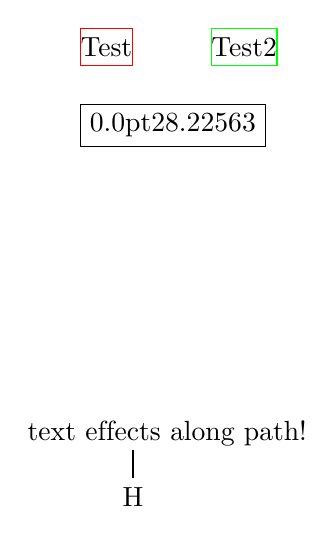
\begin{tikzpicture}[decoration={text effects along path,
	text={text effects along path!},
	text effects/.cd,
	path from text, character count=\i,
	characters={text along path,text depth=0ex,name=\i}},
]

	\path [decorate, text effects={characters/.append={}}] (0,0);
	
	\node[below=10pt of 10] (10i) {H};
	\draw[solid] (10) -- (10i);
		
	\node [inner xsep=0pt,draw=red] (A) at (1,5) {Test};
	\node [inner xsep=0pt,draw=green] (B) at (2.75,5) {Test2};
	\path let  \p1 = ( $(A.east) - (B.west)$ ), \n1 = {veclen(\x1,\y1)} 
	in \pgfextra{
		    \pgfmathparse{scalar(\n1)<10 ? 1 : 0}
			\ifthenelse{\pgfmathresult>0}{\pgfmathsetlengthmacro{\myshift}{5em}}{\pgfmathsetlengthmacro{\myshift}{0pt}}
		} node[below=of A.west,draw,xshift=\myshift,anchor=west] {\myshift \pgfmathparse{scalar(\n1)}\pgfmathresult};
	\end{tikzpicture}   
\end{document}